\documentclass[article,12pt,onesidea,4paper,english,brazil]{abntex2}

\usepackage{lmodern, indentfirst, nomencl, color, graphicx, microtype, lipsum,textcomp}			
\usepackage[T1]{fontenc}		
\usepackage[utf8]{inputenc}		

\setlrmarginsandblock{2cm}{2cm}{*}
\setulmarginsandblock{2cm}{2cm}{*}
\checkandfixthelayout

\setlength{\parindent}{1.3cm}
\setlength{\parskip}{0.2cm}

\SingleSpacing

\begin{document}
	
	\selectlanguage{brazil}
	
	\frenchspacing 
	
	\begin{center}
		\LARGE SOPH - PORTO ORGANIZADO DE PORTO VELHO: análise da demanda de maquinário utilizado para o transporte e/ou armazenamento das cargas1\footnote{Projeto de Pesquisa realizado dentro da Grande Área Organizações Públicas com apoio e supervisão do IFRO Campus Porto Velho Zona Norte.}
		
		\normalsize
		Daiana Cavalcante Gomes\footnote{Colaboradora, daianasabina@gmail.com, Campus Porto Velho Zona Norte.} 
		Jenerson Queiroz Lima Duarte\footnote{Colaborador, jenersonduartee@gmail.com, Campus Porto Velho Zona Norte.} 
	Diego da Cruz Lopes\footnote{Colaborador, dig.crz@gmail.com, Campus Porto Velho Zona Norte.} 
	Adonias Soares da Silva Junior\footnote{Orientador, adonias.silva@ifro.edu.br, Campus Porto Velho Zona Norte.} 
	\end{center}
	
	% resumo em português
	\begin{resumoumacoluna}
		Com a crescente demanda de exportação fluvial que o município de Porto Velho possui, esta pesquisa objetivou conhecer o sistema de logística e administrativa utilizada pela Sociedade de Porto Hidrovias do Estado de Rondônia- SOPH. O porto tem sido responsável pelo crescimento econômico e fortalecimento da economia rondoniense ao longo dos últimos. As metodologias utilizadas foram de levantamento bibliográfico, visita técnica, entrevista estruturada e questionários. Dar- se-á como resultado da pesquisa que SOPH possui uma estrutura que precisa ser melhorada, como o seu corpo de funcionários, a estrutura física, a gestão administrativa e a gestão gerencial de informação para que suas atividades sejam realizadas de forma efetiva e eficaz.
		
		\vspace{\onelineskip}
		
		\noindent
		\textbf{Palavras-chave}: Porto. Logística. Rio Madeira.
	\end{resumoumacoluna}
	
	\textual
	
	\section*{Introdução}
	
	Texto da introdução.O presente estudo pretendeu através da pesquisa de campo e de conhecimentos prévios adquiridos na disciplina de Gestão Patrimonial e Logística aplicada aos discentes do terceiro período do curso de Gestão Pública, apontar os meios utilizados para o transporte e/ou armazenamento das cargas, e, quais as máquinas envolvidas na logística e funcionamento do porto de Porto Velho, administrado pela empresa Sociedade de Portos e Hidrovias do Estado de Rondônia
	– SOPH. De acordo com a Secretaria de Portos - SEP, da Presidência da República, as novas perspectivas para o setor portuário que atuam com aumento expressivo no fluxo de mercadorias nos portos (acima de 10\% ao ano), cabendo ao Governo revisar e fiscalizar o planejamento do setor. O presente trabalho buscou o conhecimento acerca do maquinário utilizado pelo porto a fim de suprir a demanda. A visita técnica dos discentes evidenciou parte das estruturas e máquinas pertencentes ao porto, de forma que o total das estruturas foi evidenciado pelo Plano de Desenvolvimento e Zoneamento do Porto de Porto Velho – PDZ, 2016.	
	\section*{Material e Método}
	
O universo da pesquisa foi a SOPH, a pesquisa realizada foi de campo onde busca enfatizar os mecanismos utilizados para o transporte e armazenamento das cargas, quais as máquinas envolvidas na realização destas atividades e a execução administrativa executada por eles. As metodologias utilizadas foram de levantamento bibliográfico, entrevista estruturada e questionários.
	
	\section*{Resultados e Discussão}
	
	O porto Organizado de Porto Velho conta com uma área de cerca de 117,000 m², a SOPH movimenta de pouco mais de 3.000.000 t de carga anuais, sendo que seus principais produtos são o milho e a soja. Possui três locais para acostagem: o cais flutuante, as rampas Roll-on/Roll-off (Ro-Ro) e o pátio das gruas, conforme ilustra a figura a seguir:
	
	\begin{figure}[!h]
		\centering
		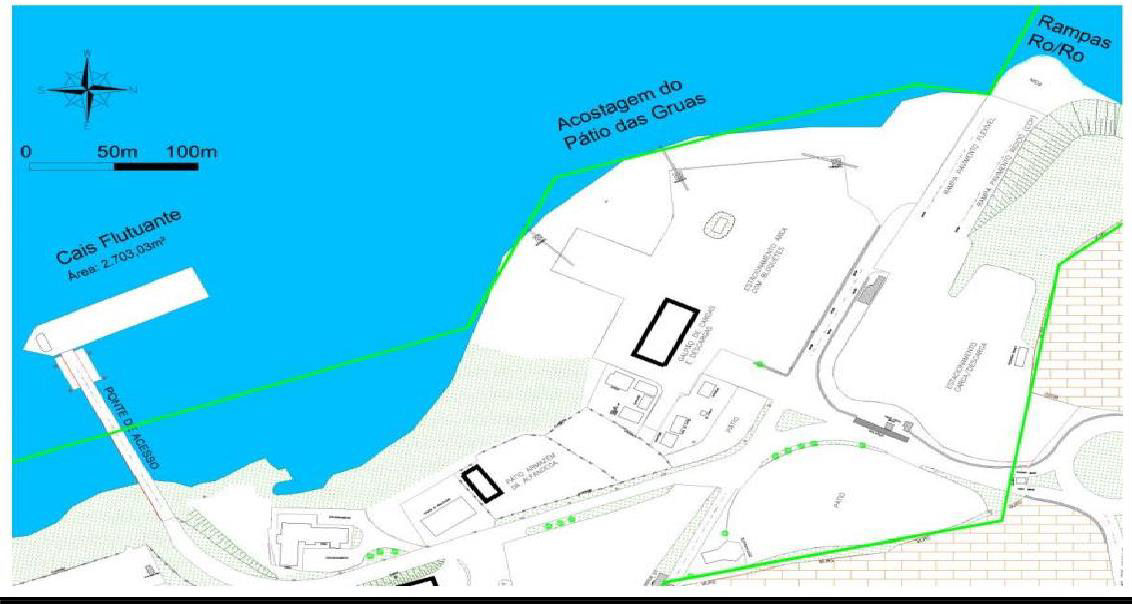
\includegraphics[width=.8\linewidth]{pip-178-01}
		\caption{Locais de Acostagem do Porto Público de Porto Velho (GOVERNO DO ESTADO DE RONDÔNIA, 2013b, apud LABTRANS).}
	\end{figure}

O cais flutuante possui 25 m de largura por 110 m de comprimento, sendo ligado à margem por uma ponte metálica de 113,5 m de vão. Pode comportar até duas balsas em cada lateral e uma balsa na extremidade de jusante. Sua área total é de 2.703,03 m².

A acostagem próxima ao pátio das gruas ocorre em barranco de talude alto e estável. Como há três guindastes, são considerados três pontos de acostagem para balsas. A movimentação de carga é feita diretamente da balsa até o pátio por meio do guindaste.

As estruturas Ro-Ro são formadas por duas rampas de concreto com capacidade de atracação para duas balsas simultaneamente. O local é dotado de estruturas metálicas do tipo charriot dando acesso ao pátio. Trata-se de rampa metálica que possibilita a transição entre a rampa de concreto e a balsa.

As instalações de armazenagem consistem em três armazéns, cinco pátios descobertos e as instalações do Complexo Hermasa. A área do terminal arrendada à Hermasa possui 40.000 m². Essa área contém quatro silos verticais com capacidade estática de 10.000 t cada, estocando soja em grãos e milho. A carga é levada ao cais flutuante por meio de esteiras.

	\section*{Conclusões}
	
Através de documentos de referências ao Porto foi possível concluir que o Porto Organizado de Porto Velho supre a demanda de cargas diárias, sendo capaz de escoar a produção do estado e a produção do noroeste do estado de Mato Grosso (Agroeste, 2011). Conforme SCHUINDT (2016), o porto tem registrado em média a movimentação de 300 mil toneladas de cargas/mês e com capacidade de até cinco milhões de toneladas/ano, corresponde a 30\% do transporte de navegação interior, conforme Resolução da ANTAQ n.º1864 de 04 de novembro de 2010, Art.1º, estabelece os procedimentos e critérios para o afretamento de embarcação para operar na navegação interior; e Art. 3º, estabelece que a navegação interior é a realizada em hidrovias interiores em percurso nacional ou internacional. Esse transporte acontece em grandes rios do interior do país ou em países vizinhos, onde acontece a navegação de balsas e barcos que transportam um grande volume de carga.
	
	\section*{Instituição de Fomento}
	
	O Instituto Federal de Educação, Ciência e Tecnologia de Rondônia, Campus Porto Velho Zona Norte, possibilitou a pesquisa, juntamente com a Sociedade de Porto Hidrovias do Estado de Rondônia- SOPH.
	
	\section*{Referências}
	
	\sloppy
	
\noindent Agroeste. Notícias de Mercado. Do silo até o exterior: conheça a rota da soja que vem do Norte do país. 2011. Disponível em:
<http://www.agroeste.com.br/noticia/18/do-silo-ate-o-exterior-conheca-a-rota-da- soja-que-vem-do-norte-do-pais>. Acesso em: julho de 2016.

\noindent BRASIL. ANTAQ. Plano Mestre do Porto de Porto Velho. Disponível em:
<http://www.portosdobrasil.gov.br/assuntos-1/pnpl/arquivos/planos-mestres- sumarios-executivos/se473.pdf>. Acesso em: junho de 2016.

\noindent BRASIL. Resolução Nº 1864 - ANTAQ, DE 4 de Novembro DE 2010. Disponível em:
<http://www.antaq.gov.br/Portal/pdfSistema/Publicacao/0000004340.pdf>. Acesso em: agosto de 2016.

\noindent BRASIL. Portal do governo do estado de Rondônia. SOPH. Disponível em:
<http://www.rondonia.ro.gov.br/soph/ >. Acesso em: junho de 2016.

\noindent BRASIL. Portal do governo do estado de Rondônia. SOPH. Disponível em:
<http://www.rondonia.ro.gov.br/soph/sobre/sobre-a-soph/ >. Acesso em: junho de 2016.

\noindent BRASIL. Portal do governo do estado de Rondônia. Plano de Desenvolvimento e Zoneamento do Porto de Porto Velho - PDZ. 2016. Disponível em:
<file:///C:/Users/80393489272/Downloads/PLANO-DE-DESENVOLVIMENTO-E- ZONEAMENTO-DO-PORTO-DE-PORTO-VELHO-Vs.final\_.pdf>. Acesso em: agosto de 2016.


\noindent CASTRO, Arnaldo Alves de. et al. Crescimento da Economia do Estado de Rondônia Movimentada Através do Porto Graneleiro de Porto Velho. XIII Encontro Latino Americano de Iniciação Científica e IX Encontro Latino Americano de Pós-Graduação. Universidade do Vale do Paraíba. 2011. Disponível em:
<http://www.inicepg.univap.br/cd/INIC\_2011/anais/arquivos/RE\_0756\_1042\_01.pdf>. Acesso em: agosto de 2016.

\noindent SCHUINDT, Rafaela. Porto público disponibiliza áreas para contratos de uso temporário em Porto Velho. Portogente. Notícias Corporativas. 2015. Disponível em: <https://portogente.com.br/noticias-corporativas/90051- Porto\%20p\%C3\%BAblico\%20disponibiliza\%20\%C3\%A1reas\%20para\%20contratos
\%20de\%20uso\%20tempor\%C3\%A1rio\%20em\%20Porto\%20Velho>. Acesso em: julho de 2016.
	
\end{document}
